\section{銀河の「進化」とは}

銀河は進化する。
この事実は、銀河研究が本格化した1970年代後半から現在に至るまで、銀河物理学の研究の
駆動力であり続けている。
にもかかわらず、銀河がどのように形成され、進化してきたかは定量的にはまだ解明にはほど遠い。
銀河の進化とは具体的に何を指すだろうか?

銀河を特徴づける物理量には実に様々なものがある。
質量に関連する諸量から見ていこう。
ダークマターを含む全質量(力学質量)、バリオンの質量、そのうちの
星が占める質量、様々な相のガスの質量(電離ガス質量、中性ガス質量、分子ガス質量)、
そして銀河を形作る星が単位時間にどのくらいの質量形成されるかを表す星形成率、星形成の結果
生成され、銀河の星間物質に供給される重元素の質量(金属量)、重元素が固体微粒子(ダスト)の
存在形態を取る量(ダスト量)と、これだけでも多くの物理量がある。

ダークマター以外の銀河の構成要素は、基本的に複雑かつ多様な輻射過程を通じて電磁波を放射する。
その結果、銀河は様々な波長の電磁波の形でエネルギーを放出している。
銀河全体の光を積分したときの単位時間、単位波長当たりのエネルギー放射量を銀河の単色光度(monochromatic 
luminosity)と呼ぶ。
単色光度(あるいは観測者が受けるフラックス密度)を波長の関数としてあらわしたものをスペクトルエネルギー
分布(SED)と呼ぶ\footnote{単にスペクトルと呼ぶ場合もあるが、波長分解能が高い場合を特に差していることが
多い。これに対してSEDというときは単色光度の概形を指している。}。
銀河の光度は波長に強く依存し、また銀河の形態(渦巻、楕円、不規則など)や星形成率、重元素量とも
密接に関連している。
X線は銀河内の星の残骸(X線連星)やブラックホールへの質量降着によるエネルギー解放現象(活動
銀河核AGNと呼ばれる)、あるいは銀河の高温ガスから放射される。
紫外線は新しく形成された大質量星、そして星の進化の最終段階である白色矮星といった高温の星からの
放射の集積である。
可視光線および近赤外線は質量の小さな星まで含めたあらゆる星の連続光、そして電離ガスからの輝線、
場合によってはAGNからの熱放射が寄与する。
中間赤外線、遠赤外線は銀河にある様々なサイズ、組成のダスト粒子に星からの紫外線、可視光線が
吸収され、再放射されるエネルギーが支配的である。
さらに、これに原子ガスからの微細構造線や分子輝線が加わる。
サブミリ波、ミリ波も同様にダスト放射が卓越するが、これに電離領域の自由電子による熱制動放射も
加わる。
ミリ波よりも長波長の電波では、熱制動放射よりも超新星残骸などの磁場による磁気制動
放射(シンクロトロン放射)が卓越する。
また、この波長では中性水素の電子と陽子のスピン状態に起因する波長21~cmの超微細構造線が
重要な放射である。
このほか、銀河内で生じる高エネルギー現象によるガンマ線も放射される。
そして、銀河全体の積分量だけでなく、銀河の各部分は異なったSEDを持っている。
渦巻銀河の中心、バルジ部分、円盤部では寄与する天体や卓越する輻射過程がそれぞれ異なるからである。
近年開発が進んでいる可視光・近赤外線波長域での面分光装置や、高空間分解能な観測を可能とする、
ミリ波・サブミリ波そしてセンチ波の大規模な干渉計装置である、ALMAやSKAが動き出そうとしている今、
これまで近傍銀河でしか検証できなかった、``空間分解したSED''の理解は、極めて重要な役割を果たすと
考えられる。

銀河を力学的な側面からみると、質量以外にも銀河のダークマターの角運動量、銀河の回転速度も
重要な物理量である。
SED同様、銀河を空間分解して構造に着目すると、渦巻銀河の渦状腕のパターンやその回転速度、
楕円銀河の局所的速度分散、その非等方性も銀河の内部力学を規定する。
矮小銀河の場合はコヒーレントなパターンがないことが多く、銀河の部分部分が異なった運動をして
いることも稀ではない(NGC~4449など)。
星形成に起因する超新星爆発によって、エネルギーが星間物質に与えられ、銀河の外にむけて運動する
銀河風という現象も知られている。
銀河のポテンシャルが深い場合は物質は減速し、銀河本体に戻ってくる。
これは銀河噴水(galactic fountain)と呼ばれる。
これに対し、矮小銀河のようなポテンシャルの浅い銀河では星間物質の流れは銀河の脱出速度を
超え、銀河の外に流出する。
この場合は銀河風(galactic wind)と呼ぶ。
どちらも銀河の質量収支に影響を与える、重要なガスの運動として注目されている。
後でも述べるが、銀河同士が衝突$\cdot$合体することは宇宙では頻繁に生じる。
銀河の大きさ($\sim 10$~kpc)に比べ、銀河間の平均距離がさほど大きくない($\sim 1$~Mpc)ためである。
銀河の質量に差がある場合は、小さな銀河が大きな銀河に吸収されたとみなせる。
この場合力学状態はさほど乱れないが、星形成率には強い影響を与え、また一時的に特徴的な外見を
呈する場合がある(シェル、リップル、ポーラーリングなど)。
同程度の質量の銀河が合体する場合は力学的な影響は極めて強く、もともと持っていた形態は
いったん完全に失われ、最終的に楕円銀河的な密度構造に落ちつくと言われている。
これに関連する有名な問題がある。
銀河を構成する星は無衝突系であることが知られており、星同士が2体散乱を起こすことは
事実上ないといってよい。
ところが、楕円銀河の密度ポテンシャルはどれも極めて似通っており、2体緩和よりもはるかに速い何らかの
緩和過程を考えなければ観測が説明できない。
この問題は現在も完全には解決されていないが、「激しい緩和過程」(violent relaxation)と呼ばれる
統計力学的過程が考えられている。
このような過程の結果、衝突銀河の最終的な``平衡''形状は楕円銀河の密度プロファイルとなる。
しかし実際の銀河は星だけではなく、衝突系であるガスも含んでいるため、星のみの系同士の合体とは異なる結果を生じる可能性もある。
例えば、ガス成分の多い銀河同士の合体(gas-rich merger)では、合体後に円盤銀河になりうる、という結果を報告している研究がある\citep{2002MNRAS.333..481B, 2005ApJ...622L...9S, robertson2008, 2009ApJ...691.1168H}。
そのため、衝突銀河のガスの分布$\cdot$運動
などの情報を調べることは、銀河進化を理解する上で極めて重要である。

これらに加え、これまで直接観測は難しかった銀河外からのガス降着や、古くて新しい問題として
知られる銀河への環境の影響(環境効果)も重要な量であろう。
環境効果が銀河の形態や性質に影響を与えることは様々な観測から知られており、今後も新たな
事実が発見されると期待される。

銀河の進化とは、これら実に多彩な物理量が宇宙年齢とともに変化していく現象を指す。
厳密には、1個の銀河に着目したときの物理量の時間変化、いわば銀河の個人的ヒストリーと
各宇宙年齢で統計的に見たときの銀河の平均的物理量の変化、つまり社会的ヒストリーの
2つの側面がある。
銀河進化研究では必要に応じてこの2つの立場を使い分けている。
宇宙論的な文脈からは、ダークマターが重力相互作用し、その構造の進化のなかで銀河が形成、
進化してゆくという立場から研究が進められる。
この場合は力学的な進化が重要である。
しかし、銀河の分野で最も注目されているのは、最初のガス塊から星が生まれ、そして初代の星が
死ぬことで重元素が供給され、次世代の星形成が促進されてゆくというサイクル、すなわち
星形成進化である。
化学組成もこれに伴って変化してゆくので、重元素量の進化のことは化学進化という特別な
用語で呼ばれる\citep{tinsley1980}。
これらに加え、最近では積分した星質量の進化も重視されている。
銀河全体の進化だけでなく、たとえば矮小銀河の質量降着や銀河になっていない残存ガスが
大規模構造のフィラメントから降着してくるなどの過程によって、銀河のバルジ-ディスク比も
進化してゆく。
銀河合体は劇的な形態の変化をもたらし、これも銀河進化の重要な側面とみなせる。
銀河の中心部には大質量ブラックホールが存在していることが多いが、このブラックホールへの質量降着が
時間変化することで、AGN活動性も進化する。
さらに、中心核ブラックホールとバルジの間に相関が存在することから、銀河の進化とブラックホールの
進化も関連していることが示唆されている\citep[e.g.][]{magorrian1998}。
これは銀河とブラックホールの共進化(co-evolution)として知られている現象である。
銀河進化という言葉は、このようなイメージでとらえるのがよいであろう。

ここ10年で、多波長による銀河探査が飛躍的に進展し、宇宙年齢の非常に早い時期まで
観測データが揃うようになってきた。
これによると、銀河の進化は上に述べた様々な物理量のうち、基本的に2つの物理量で決まっているらしい
ことが見えてきつつある。
銀河の星質量と、局所的な環境である。
現在標準となっている、宇宙項のある冷たいダークマター宇宙モデル($\Lambda$CDMモデル)が
予言する階層的構造形成シナリオでは、小さな構造単位(ダークハロー)が合体することによって
より大きなダークハローが形成され、ダークハローの重力ポテンシャル環境の中で銀河が形成されると
考えられている。
銀河形成期以前の宇宙では、バリオンはほぼ完全にガス相で存在する。
それが大規模構造のフィラメントに降着し、そしてハローの作るポテンシャルに落下して濃い分子雲を
作ることで星形成が始まる。
分子雲から初期質量関数に従って星が誕生する。
大質量星は温度が高く、光度も大きいため強い紫外線で周囲のガスを電離し、電離水素領域を
形成する。
これは星形成の観点からは阻害に働く高価である。
また大質量星は短いタイムスケールで超新星爆発を起こし、持っていたガスを星間空間に戻す際に
重元素やダストを供給し、それとともに熱エネルギーや衝撃波を星間物質に与える。
冷たいガスや分子雲はこのようなエネルギーインプットによって熱いガスとなり、星形成は停止して
しまう。
これに加え、AGNからの強烈な放射やジェットなども星間物質の冷却を妨げる。
これらはネガティブフィードバックと呼ばれ、星の形成が進むことで星の形成を阻害する方向に働く。
この意味で、星形成は自己制御的(self-regulating)であると言われることもある。
このように、ダークハローの影響とバリオン物質の複雑なフィードバック機構が銀河の星形成を制御しつつ
進化し、今日の銀河となるのである。
銀河の星質量の成長を完全に理解するためには、星形成の原料である中性ガスの複雑な物理
過程を解明する必要がある。
このように、銀河の形成進化と大規模構造進化の理解には、銀河中の中性ガスをなるべく多くの
銀河について、なるべく異なった様々な環境で、宇宙年齢の関数として理解することが不可欠である。

\section{銀河進化研究の現状 -- 伝統的方法論とその限界 --}\label{galaxy.s0.5}

銀河進化の星形成に関する側面は、1970年代後半にTinsleyらが銀河の星種族の進化に
基づく観測量の進化理論を提唱して以来、様々な観測量を用いて検証されてきた。
まず注目されたのが、銀河の星種族の構成である。
星の寿命が星の初期質量に強く依存することから、同時期に生まれた星の集団の色(カラー)は
大質量の星から先に死んでいくことにより、時間とともに変化する。
黎明期の銀河進化研究で重視されたのは、化学進化理論に基づく銀河のカラーの進化であった
\citep[e.g.][]{larson1974, larson1978, larson1980}。
この頃は、階層的構造形成モデルはまだ標準としての地位を確立しておらず、銀河進化は
ワンゾーンで古典的に時間進化すると扱われていた。
この場合、個々の銀河の進化 $\simeq$ 銀河の平均的進化といえる。
現代的視点からみるとまだ未成熟ではあるが、銀河の平均的進化を宇宙論的な体積平均で
捉える「宇宙の星形成史」という概念を初めて提唱したのは\citet{tinsley_danly1980}である\footnote{よく
誤解されているが、最初に提唱したのはPiero Madauでは{\bf ない}。}。
宇宙の星形成史は1990年代後半に深い銀河探査を用いて銀河の平均的進化の検証に使われ
始めて以降、爆発的な流行を呼ぶこととなった\citep[e.g.][]{lilly1996, madau1996}。
銀河のカラーに基づく進化の検証の利点はもちろん、非常に成功した天体物理理論である星の進化の
体系を用いた明快な議論ができることである。
しかし、銀河のカラーの変化は概して時間分解能が極めて低く、その年齢での星形成率を測定できない。
特に長寿命の星からの輻射が卓越してくる銀河年齢($< 数{\rm Gyr}$)では顕著である。
このため、寿命の短い大質量星起源の物理量を用いる方法がこれに取って代わることになった。

大質量星は上記のように電離水素領域(H{\sc ii}領域)を形成する。
H{\sc ii}領域では水素の電離再結合が生じるため、Lyman, Balmer, Brackett系列など
水素の再結合線が放射される。
水素の再結合線強度は電離光子の数から量子力学的に正確に計算できるため、第一原理に
基づくクリアな議論がやはり可能である。
観測から再結合線の強度を測定して電離光子の数に換算し、そして星の輻射の理論から大質量星
(OB型星)の数(あるいは総質量)に焼き直す。
これに初期質量関数を仮定することで、大質量星の総質量は全質量の星の質量に換算できる。
こうして得られた星の質量は、大質量星の寿命のタイムスケール($10^6$~yr)の時間に形成された
星の全質量、つまり星形成率を表している\citep{kennicutt1983}。
これが銀河の進化のタイムスケールに比べて十分短いことから、銀河進化を議論する主要なツールと
して広く用いられている。
水素の再結合線のうち、最も進んでいた可視光線での観測に都合がよいのがBalmer系列の
輝線(H$\alpha$、H$\beta$、H$\gamma$など)である。
Lyman系列は紫外線であり、赤方偏移が高い銀河では可視光で観測できるため、10~mクラスの
光学望遠鏡が建造されるようになってから銀河進化研究によく用いられるようになった。
また、大気吸収や夜光によって地上空の観測が難しかった近赤外線のBrackett系列も、観測
装置の発展により今日では星形成率の研究に用いられている。
赤方偏移が1--2付近の銀河ではBalmer系列がこの地球大気による邪魔の多い波長にシフトするため
観測が困難であることから長く「赤方偏移砂漠」(redshift desert)と呼ばれていたが、同様に
近赤外線観測装置の発展によりこの問題も解決に向かっている。
ところが、水素再結合線による星形成の評価は万能ではない。
\citet{kennicutt1983}の中ですでに議論されているように、銀河の星形成は必ずダストの
生成を伴う。
可視光線および紫外線はダストの減光\footnote{ダスト粒子による散乱と吸収の効果の総称をこう呼ぶ。}の効果を
強く受けるため、観測量からそのまま算出した星形成率は常に過小評価である。
この問題は早い時期から認識されていたものの、銀河進化、特に紫外線に根拠を置く研究者の間では
軽視され続け、その結果銀河の星形成進化についての理解の混乱を引き起こすことになった。

ダスト粒子は星が形成され、大質量星が超新星爆発を起こすタイムスケールで生成される。
このためダストは星形成領域には必ず存在している。
ダストが吸収した紫外線のエネルギーはダスト粒子からの熱放射として主に中間--遠赤外線で再放射
されるので、ならばむしろ赤外線放射光度を大質量星からの電離光子の指標として用いることが
考えられる\citep[e.g.][]{1998ARA&A..36..189K}。
ダストによる吸収が顕著な銀河では、この方法は星形成の指標として有効である。
遠方宇宙においてダストで強い吸収を受け、巨大な赤外線光度を持つ銀河が発見されたことで、
星形成率の指標としての赤外線は急激に注目されることになった\citep[e.g.][]{hughes1998}。
高光度赤外銀河と呼ばれるこの種族は、1個当たりの星形成率が極端に高い(100--1000~$M_\odot\,{\rm yr}^{-1}$)
ため、宇宙の星形成率への寄与が大きい可能性が指摘され、星形成率はむしろ赤外線のみで
測定すれば足りるという極端な見方をする研究者も出てきた。
しかし当然ながら紫外線のみ、赤外線のみではどちらも不十分な情報しか得られないことは自明である。
\citet{takeuchi2005}は$0 < z < 1$の宇宙で紫外線と赤外線の光度関数をもとめ、これらを積分することで
全星形成率への双方の寄与を評価した。
その結果、近傍宇宙ではほぼ同じ寄与となるものの、$z=1$の宇宙では90~\%以上の星形成がダストで
隠されており、赤外線でしか観測できないことを見出した。
この結果はその後の研究により$z \simeq 4$まで検証され、$1 < z < 3$の宇宙ではこの隠れた星形成が
支配的であることが確定的となった\citep[e.g.][]{cucciati2012, burgarella2013}。
とはいえ、双方の情報を用いた星形成率指標が理想的であることは言うまでもなく、現在ではそのような
指標がいくつか提唱され、評価されている\citep[e.g.][]{kennicutt2009,takeuchi2010,murphy2011}。
このうち、電波連続波もダストの影響を受けない星形成率の指標として使われており、電波連続波で探る銀河進化は、
SKAの重要なサイエンステーマの一つである (詳細は\S~\ref{sec:continuum}参照)。

その他の星形成率を評価するための観測的指標としては、X線連星起源の光度、H{\sc ii}領域からの禁制線
([O{\sc ii}]など)の光度、多環式芳香族炭化水素のバンド輝線光度、非電離紫外線連続光光度や
シンクロトロン放射光度などが用いられている。
ところが、これらはすべて星形成率を測る指標であり、銀河形成と成長のキーである「ガスから星への変換」に
ついては何も語ってはくれない。
これに対し、電波天文学では分子輝線を用いた分子ガス量が星形成に関連する測定量として
精力的に研究されてきた。
こちらはある時刻における銀河が持つ「星形成の材料」の量を示している。
これと星形成率を組み合わせることで、ガスから星への過程を議論することができる。
しかし、分子輝線はすでに分子雲になったガスをトレースするのみであり、更にこれをおしすすめて中性ガスまで
含めた議論をする必要がある。
これまではH{\sc i}の21~{\rm cm}輝線が観測できる赤方偏移がほぼ近傍宇宙に限られていたため、銀河進化の
観点から議論されることは稀であった。
SKAはこれを可能にし、銀河進化研究に絶対的なブレイクスルーを与えることになる。


\section{銀河進化研究の現状 -- 銀河におけるHIガス --}\label{galaxy.s1}

%%%%%%%%%%%%%%%%%%%%%%%%%%%%%%%%%%%%%%%%%%%%%%%%%%%%%%%%%%%%%%%%%%%%%%%%%%
\subsection{水素原子と水素分子}\label{sec:HI_H2}
%%%%%%%%%%%%%%%%%%%%%%%%%%%%%%%%%%%%%%%%%%%%%%%%%%%%%%%%%%%%%%%%%%%%%%%%%%

銀河において星形成の材料となるのは分子ガスである。銀河系では、
星間物質のうち質量の約半分が分子ガス、特に水素分子(H$_2$)ガスになっていることが知られている。
この小節では銀河における水素分子の生成および解離と、水素分子と水素原子(H {\sc i})
の割合について述べる。
SKAの観測では、原子ガスが重要な観測対象となるが、原子と分子の二相は下で
見る様に密接に関係しており、両方の理解が重要である。

\subsubsection{水素分子の生成}
銀河において、水素分子の最も基本的な生成過程は2つの水素原子による共役反応で、電子や陽子を触媒として起こる。この共役反応では水素分子の生成に伴って多量の発熱エネルギーが生じる。この発熱エネルギーを捨て去られない限り反応は逆戻りするため水素分子は生成できない。
水素分子生成に伴う発熱エネルギーを捨て去るためには3つの水素原子による衝突反応が必要となる。この衝突反応では3つ目の水素原子が余分な発熱エネルギーを持ち去ってくれるため、水素分子を生成することができる。このような3つの水素原子による水素分子の生成は、非常に高密度な環境($n_{\text{H}}>10^8$ cm$^{-3}$)で促進される。しかし実際の銀河では、銀河系の分子雲でさえ水素原子の平均的な個数密度が$n_{\text{H}}\sim10^5$ cm$^{-3}$以下という低密度環境であるため、水素原子の衝突反応による水素分子生成はほとんど起こらない。

銀河において最も効率のよい水素分子生成は星間塵を触媒とする
方法である\citep{1963ApJ...138..393G, 1971ApJ...163..155H}。
星間塵の内部では様々な運動モードが存在している。そのため、星間塵表面で水素分子が生成されると、生成で生じた発熱エネルギーは星間塵が熱浴となって吸収してくれると考えられる。

星間塵表面での水素分子形成過程は、1) 水素原子の星間塵表面への付着過程、2) 星間塵表面での拡散過程、3) 星間塵表面での2つの水素原子の反応過程、4) 生成した水素分子の星間塵表面からの離脱過程の4つの素過程にわけて考えることができる(図\ref{fig:grain})。まず、気相中を漂っているある水素原子が星間塵の表面に付着する(過程1)。この時水素原子が星間塵に付着できるかどうかは、水素原子の星間塵への衝突エネルギーと星間塵からの脱出エネルギーのバランスで決まる。衝突エネルギーが星間塵に十分に吸収され、星間塵表面からの脱出に要するエネルギーを満たさなければ水素原子は付着できる。
付着した水素原子と星間塵表面の間に働く結合力(Van der Waals力)は弱い。そのため、水素原子は星間塵表面上を動き回り、やがてポテンシャル場の井戸に落ち込む(過程2)。
次に別の水素原子が星間塵表面に付着し、最初の水素原子同様に表面上を動き回る。しばらくすると、この水素原子はポテンシャル場にいる最初の水素原子と出会い、水素分子を生成する(過程3)。分子動力学シミュレーションによると、この水素分子生成の反応には2つのパターンが見られる\citep{1999MNRAS.306...22T}。
1つ目は上述の星間塵表面上での2つの水素原子により引き起こされるパターン、2つ目は星間塵表面に付着している水素原子へ気相中の別の水素原子が直接衝突をして反応を起こすパターンである。
いずれかの反応によって生成された水素分子は、星間塵表面における結合エネルギーを切り、気相として星間塵表面から離脱する(過程4)。
星間塵表面での水素分子の生成率は、太陽系近傍の分子雲で$k\sim 3 \times 10^{-17} \; \mbox{cm}^3\, 
\mbox{s}^{-1}$であるといわれている\citep{1975ApJ...197..575J}。


%%% Figure
\begin{figure}[tbp]\label{fig:grain}
\begin{center}
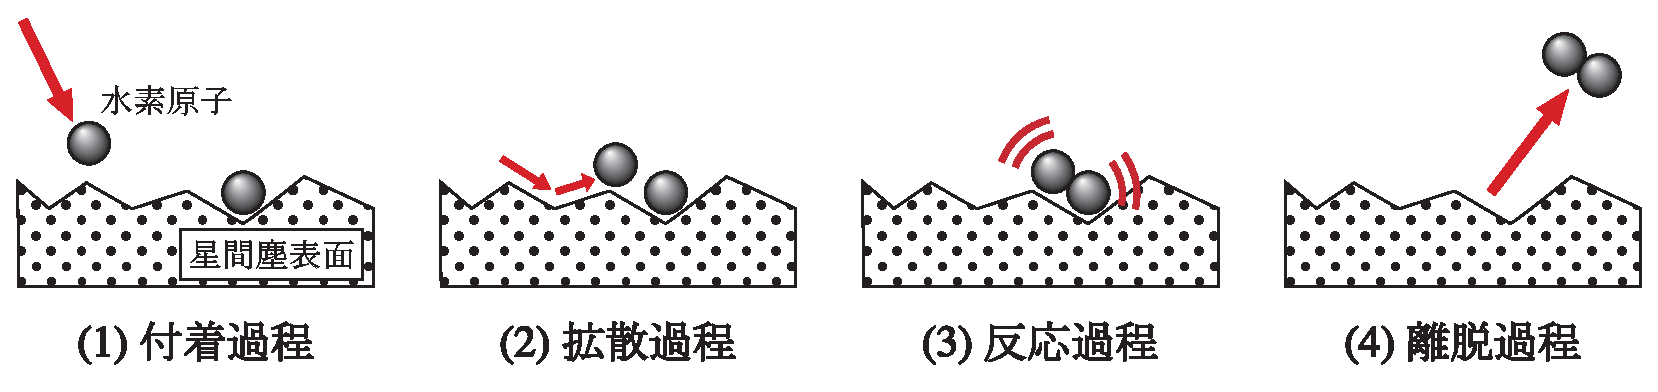
\includegraphics[width=\linewidth]{galaxy/h2form.eps}
\end{center}
\caption{星間塵表面における水素分子生成の4つの素過程(高橋 2000)。}
\end{figure}
%%%

\subsubsection{水素分子の解離}

一度生成された水素分子も何らかの原因で解離され、再び水素原子に戻ることがある。この水素分子の解離を引き起こす原因は大きく3つあげられる。
まず1つ目は、主にO型星と一部のB型星から放射される$11.2-13.6$ eVの紫外光子(Lyman-Werner光子)による光解離である。 このような放射場の周囲では、水素分子のみで構成された分子雲は光解離によって水素分子から水素原子へ解離されてしまう。
しかし、分子雲が非常に高い柱密度をもつ場合($N_{{\rm H}_2}>10^{14} \; \mbox{cm}^{-2}$)、その内側は自己遮蔽によって光解離を免れる\citep{1996ApJ...468..269D}。
また、分子雲中に星間塵が含まれていた場合も紫外光子は星間塵によって吸収・散乱されるため、分子雲の内側は光解離の影響を受けない。このような光解離を免れた分子雲の内側で新しい星が形成されると考えられている。

2つ目は$1\mbox{--}100$~MeV程度の陽子である宇宙線による解離である。
宇宙線は星間塵の影響を受けず、分子雲を貫くことができる。そのため、分子雲の中心部の水素分子を電離させる。この反応は水素分子の宇宙線電離とも呼ばれる:
	\begin{eqnarray}
		\text{H}_2		+ (宇宙線) 	& \rightarrow & \text{H}^+_2 	+ e^-	+ (宇宙線) .
%									& \rightarrow & \text{H}^+		+ H		+ e^-	.
	\end{eqnarray}
この反応によって生じたH$_2^+$イオンは周囲の水素分子とただちに反応してプロトン化水素分子(H$^+_3$)を生成する。
	\begin{eqnarray}
		\text{H}_2^+	+ \text{H}_2	& \rightarrow & \text{H}^+_3 	+ \text{H}
	\end{eqnarray}
分子雲では、宇宙線電離によって生成されたH$^+_3$が他分子の生成に寄与することが知られている\citep{johnsen}。

3つ目の水素分子の解離過程は高温$\cdot$高密度な星間空間における衝突解離である。中性な星間空間では、水素分子の衝突解離は水素原子、ヘリウム原子、水素分子によって引き起こされる。
電離領域では、電子や陽子が水素分子の衝突解離を誘発する。また、速度が$v_s > 20\; \mbox{km} \, \mbox{s}^{-1}$をもつ衝撃波領域でも衝突解離が生じることが知られている\citep{1977ApJ...216..713K, 1977ApJ...217..442L}。
しかしこの衝突解離は水素分子解離の原因としての寄与は小さいと考えられる。理由としては、衝突解離によって水素分子生成で生じる熱エネルギーが効率よく捨て去られたり、星間空間中の金属による冷却を受け、水素分子の解離よりも生成が促進されるためである\citep[e.g.][]{1963ApJ...138..393G}。

\subsubsection{銀河における水素分子と水素原子}

銀河における水素分子と水素原子の割合(分子比率:$f_{\text{mol}}\equiv \rho_{{\rm H}_2} / \rho_{{\rm total}}$, $\rho_{{\rm total}}=\rho_{{\rm H}_2}+\rho_{\rm HI}$)は、水素分子の生成と解離のバランスで決まる。
\citet{1993ApJ...411..170E}は、$f_{\text{mol}}$が分子雲にかかる様々な圧力、紫外光子の放射場、金属量の関数として記述される解析的な1次元のモデルを提案した。
\citet{2008ApJ...689..865K}では、\citet{1993ApJ...411..170E}の分子雲を球対称モデルとして扱い、星間塵による水素分子生成をパラメーターとして加えた多次元の解析モデルを提案した。
これらのモデルは、銀河系や近傍銀河の観測結果をよく説明している\citep{1995A&A...296...33S, 1995A&A...304....1H, 2004ApJ...612L..29B, 2008AJ....136.2782L}。

観測的な$f_{\text{mol}}$の検証は、主に、銀河系や近傍銀河の$^{12}$CO($J=1-0$)輝線(2.6~mm)とH\,{\sc i}輝線(21~cm)の観測データをもとに行われている。$^{12}$CO($J=1-0$)輝線の観測からは輝線強度と水素分子柱密度の変換係数($X_{\text{CO}} \;\mbox{[cm}^{-2} \mbox{(K km s}^{-1})^{-1}]$)を介し水素分子の面密度が、H\,{\sc i}輝線の観測からは水素原子の面密度が得られる。これら面密度の比から$f_{\text{mol}}$は見積もられる。
円盤銀河で代表される晩期型銀河では、銀河全体として$f_{\text{mol}}\sim 25 \mbox{--} 30\; \%$に
なると報告されている\citep{2014A&A...564..66B}。
さらに、晩期型銀河における$f_{\text{mol}}$の動径分布を調べると、銀河中心から動径方向に減少することが知られている\citep[e.g.,][]{2012ApJ...756..183B, 2014PASJ...66...66T}。
図\ref{fig:leroy}は晩期型である渦巻銀河(NGC 628)における、中心からの水素分子・水素原子面密度の動径分布を表している。
水素分子は銀河中心部をピークに動径方向に面密度が小さくなっていく。一方、水素原子は銀河中心部では面密度が小さく、数kpc外側から(図\ref{fig:leroy}では半径$100''$付近)動径方向に面密度は徐々に大きくなる。そのため、晩期型銀河の$f_{\text{mol}}$は銀河中心部で1に近く、外側にいくにつれて小さくなるような分布を示す。

次に、水素原子から水素分子へ遷移する密度について記述する。
解析的な理論モデルによると、太陽の金属量をもつ球対称な分子雲の中では、光解離からの遮蔽が水素原子の面密度で$\Sigma_{\text{HI}} \approx 10\; M_\odot \mbox{pc}^{-2}$付近(柱密度で$N_{\text{H}}\sim 10^{21}\;
\mbox{cm}^{-2}$程度)で効くことが示唆されている\citep{2009ApJ...693..216K}。
水素分子の生成/解離を組み込んだ銀河形成進化の数値シミュレーションにおいても、同様の金属量をもつ銀河では$N_{\text{H}}\sim 10^{21} \; \mbox{cm}^{-2}$でほぼ全ての水素原子は水素分子へと遷移する
\citep[e.g.,][]{2006ApJ...645.1024P, 2009ApJ...697...55G}。
これら理論研究による予言値とほぼ等しい値が、太陽と同程度の金属量をもつ近傍の晩期型銀河の観測から得られている\citep[e.g.,][]{2002ApJ...569..157W, 2008AJ....136.2846B}。

しかし、水素分子へ遷移する柱密度は金属量によって変わりうる。Gnedin et al. (2009)では、金属量が低いほど水素分子へ遷移する柱密度が高くなることを示唆した。彼らのシミュレーションの中では金属量が低いと光解離を遮蔽する星間塵が少なくなる。そのため、光解離からの遮蔽が効く柱密度は高くなる。同様の結果は他の理論モデルや近傍銀河の観測からも得られており\citep[e.g.,][]{2009ApJ...693..216K, 2010ApJ...709..308M, 2010ApJ...722..919F, 2013ApJ...777L...4W, 
2014MNRAS.442.2780R}、金属量は水素原子から水素分子への遷移において鍵となるパラメーターと言える。

%%%%%%%%%%%%%%%%%%%%%%%%%%%%%%%%%%%%%%%%%%%%%%%%%%%%%%%%%%%%%%%%%%%%%%%%%%
\subsection{渦巻銀河のHIガス}
\label{sec:spiral}
%%%%%%%%%%%%%%%%%%%%%%%%%%%%%%%%%%%%%%%%%%%%%%%%%%%%%%%%%%%%%%%%%%%%%%%%%%

渦巻銀河の中性水素ガス(H\,{\sc i}ガス)の観測は1950年代に遡る。以来、電波単一鏡や干渉計
\footnote{2014年現在科学運用されている望遠鏡としては、電波単一鏡ではGreen Bank Telescope、Areciboが、干渉計ではVery Large Array (VLA)などがある。}
によって、非常に近傍($\sim50$ kpc)から、100 Mpc以上($z>0.024$)の銀河に至るまで広く観測されている。本小節では渦巻銀河におけるH\,{\sc i}ガス観測によってもたらされた物理的な理解についてまとめる。


\subsubsection{空間分布}\label{sec:distribution}
渦巻銀河におけるH\,{\sc i}ガスの分布には大きく3つの特徴が見られる。
1つ目の特徴は銀河中心部に見られる穴である。一般的に銀河中心部は高密度である。そのため、ほぼ全ての水素原子が水素分子に遷移してしまい、H\,{\sc i}ガスがほとんど存在していないことに起因していると考えられている($\S$\ref{sec:HI_H2}参照)

2つ目の特徴は、H\,{\sc i}ガスは可視光観測で得られる円盤部より顕著に広がって分布していることである\citep[e.g.,][]{1983IAUS..100...55S, 2008AJ....136.2782L}。
図\ref{fig:leroy}上側のパネルには近傍渦巻銀河(NGC 628)の可視観測より得られた星、H\,{\sc i}ガス、CO観測による分子ガスの空間分布が示してある。星や分子ガスは図中の黒点線で囲まれた円内に収まるのに対し、H\,{\sc i}ガスは円のかなり外側まで広がっていることがわかる。このように多くの渦巻銀河では、H\,{\sc i}ガスは星の円盤と比べ2--3倍以上広がっている\citep[e.g.,][]{1983IAUS..100...55S}。

渦巻銀河の外側に見られる広がったH\,{\sc i}ガスのような、星の円盤周囲にあるガスは銀河周辺ガス(circum-galactic medium: CGM)と呼ばれている。
CGMは、理論的には銀河間ガスの降着や銀河からのアウトフローに関連していると考えられており\citep[e.g.,][]{2002ApJ...571...40M, 2006Natur.440..644M, 2009Natur.457..451D, 2009ApJ...703..785D, 2005ApJ...635L..13S, 2011MNRAS.415..11D}、銀河の質量獲得過程や星形成史と密接に関連した重要な研究対象となっている。CGMのH\,{\sc i}ガスの柱密度は円盤部
\footnote{渦巻銀河円盤部のH\,{\sc i}ガス柱密度は$N_\mathrm{HI}\sim10^{20\mbox{--}21}$ cm$^{-2}$程度。}
と比べ低く($N_\mathrm{HI}<10^{19}$ cm$^{-2}$)、観測的な直接検出が課題であった。しかし近年の観測装置の性能向上により、高感度のH\,{\sc i}ガス観測が可能となり、CGMの淡いH\,{\sc i}ガス($N_\mathrm{HI}\sim10^{18}\; \mbox{cm}^{-2}$)が検出され始めてきた\citep{2013Natur.497..224W, 2014AJ....147...48P}。
このデータをもとに渦巻銀河へのガスの流入の議論が行われつつある。

3つ目の特徴は、H\,{\sc i}ガスの面密度($\Sigma_{{\rm HI}} [M_\odot \mbox{pc}^{-2}]$)が渦巻銀河の外側で比較的一定になることである。銀河中心から各半径における$\Sigma_{\text{HI}}$は、中心で低く(特徴1)、半径が大きくなるにつれて急に高くなり、ある半径でピーク($\Sigma_{\text{HI}}^{\text{max}}$)となる。
その半径より外側では、$\Sigma_{\text{HI}}$の動径分布は比較的平坦になる\citep[e.g.,][図\ref{fig:leroy}下参照]{2008AJ....136.2782L, 2012ApJ...756..183B}。
$\Sigma_{\text{H\,{\sc i}}^{\text{max}}}$は高くとも$\sim10$ $M_\odot$ pc$^{-2}$程度までしかあがらない。それは、$\Sigma_{\text{H\,{\sc i}}}>10$ $M_\odot$ pc$^{-2}$ではほとんどの水素原子は水素分子に遷移してしまうためである($\S$\ref{sec:HI_H2}参照)。

%%% Figure
\begin{figure}[t]
%\vspace{-4\baselineskip}
\begin{center}
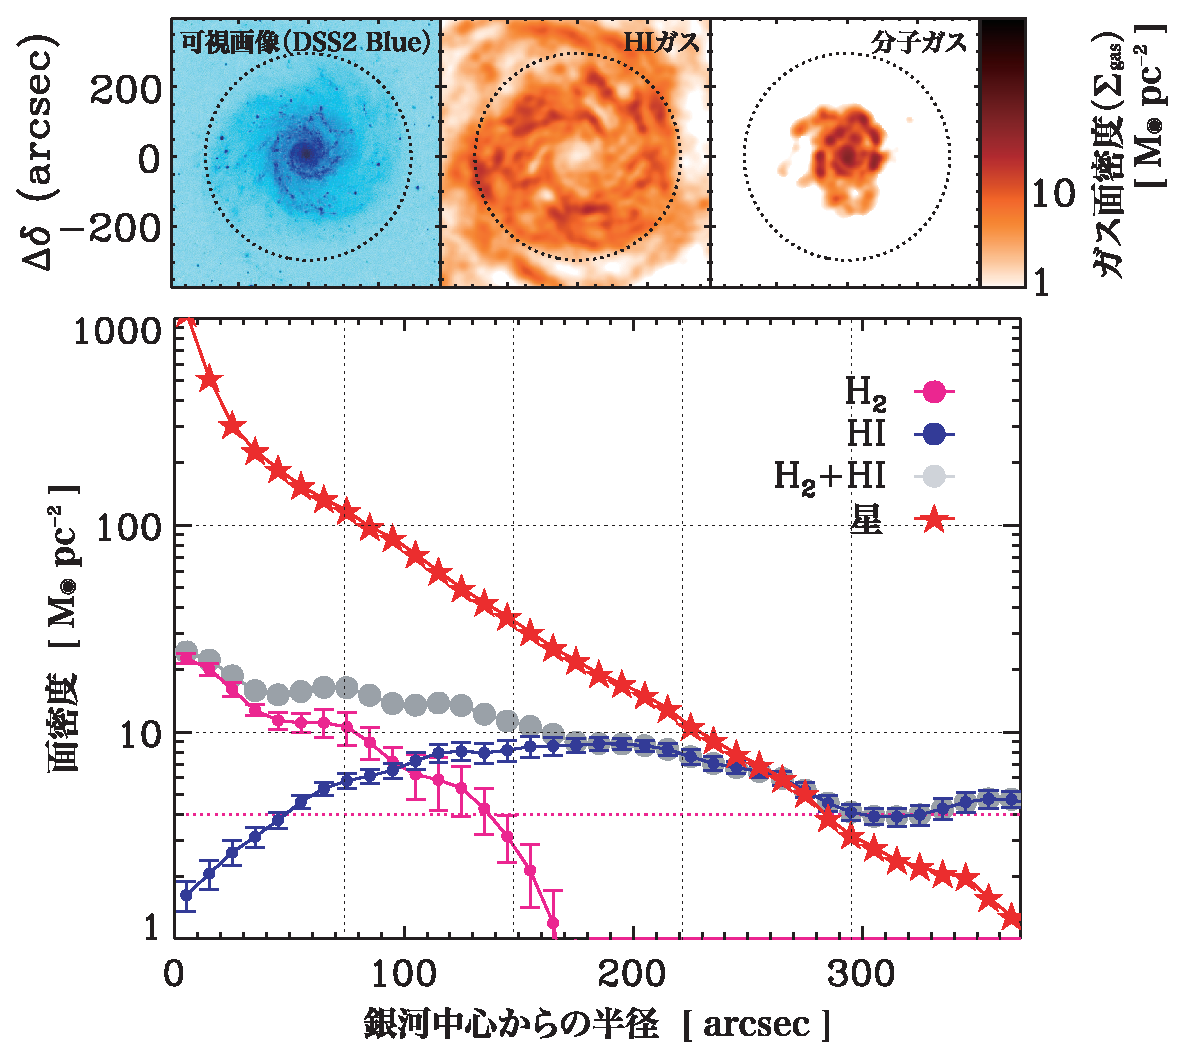
\includegraphics[width=12cm]{galaxy/Leroy08.eps}
\end{center}
\caption{NGC 628のH\,{\sc i}ガス、分子ガス、星の画像と銀河中心からの動径分布(Leroy et al. 2008を修正し転載; 可視画像はSpace Telescope Science Instituteより)。物理的なスケールとして、$1''$は約35~pcに相当する。}
\vspace{1\baselineskip}
\label{fig:leroy}
\end{figure}
%%%


\subsubsection{H\,{\sc i}ガス質量}
21~cmで観測されるH\,{\sc i}ガスは光学的に薄く、次の関係式を用いて視線方向の輝線強度($I_\mathrm{HI}\; \mbox{[K km s}^{-1}$])から柱密度$N_\mathrm{HI}$を求めることができる。
	\begin{eqnarray}
		N_\mathrm{HI}~[\text{cm}^{-2}] = 1.823 \times 10^{18} \; I_\mathrm{HI}~[\text{K km s}^{-1}] 
	\end{eqnarray}
また、得られた柱密度を銀河の全領域で積分すると、銀河におけるH\,{\sc i}ガスの総質量を求めることができる。
観測データをもとに見積もられた渦巻銀河におけるH\,{\sc i}ガスの総質量は、$M_{\text{HI}}\sim10^{8\mbox{--}10} \; M_\odot$程度となる\citep[e.g.,][]{2008AJ....136.2563W}。
なかでも$M_{\text{HI}} \sim10^{10} \; M_\odot$近い値を示す渦巻銀河は衝突している銀河であり、銀河同士の衝突や相互作用によって多くの星間物質がもたらされた結果であると考えられている。

このように見積もられた渦巻銀河のH\,{\sc i}ガスの総質量と円盤部の大きさには相関が見られることが知られている。
$\S$\ref{sec:distribution}に記したように、渦巻銀河では$\Sigma_{\text{HI}}$が外側の半径でほぼ一定となる。そこで銀河全面にわたり$\Sigma_{\text{HI}}$が一定であると見なすと、渦巻銀河のH\,{\sc i}ガス総質量は銀河の面積にほぼ比例することになる。実際に、H\,{\sc i}ガスの総質量が主に星円盤の半径に依存していることが示唆されている\citep[e.g.,][]{2012ApJ...756..183B}。


\subsubsection{力学情報}
H\,{\sc i}ガスは渦巻銀河内の広域に分布しているため、その運動情報から銀河の質量分布を求めることができる。図\ref{fig:deblok08}には様々な渦巻銀河におけるH\,{\sc i}ガスの回転速度が距離の関数(回転曲線)として示されている。回転速度の大きさは平均的に$150-300$ km s$^{-1}$と銀河によって異なるが、基本的には回転曲線は中心から外側にいくほど速くなり、ある半径でほぼ一定($v_{\text{max}}$)に達するという平坦な分布を示す\citep[e.g.,][]{1980ApJ...238..471R, 1985ApJ...289...81R,1981AJ.....86.1791B, 1987IAUS..117...67S, 1987IAUS..124..699S}。
ここでH\,{\sc i}ガスは銀河内を回転曲線に従う円運動を行なうと仮定する。
この時、銀河の質量分布に回転対称性があると仮定し、半径$r$以内に含まれる質量を$M$($r$)、$r$での回転速度を$v(r)$とすると、重力と遠心力のつり合いから
%この時、銀河の質量分布が球対称であると近似すると、半径$r$以内に含まれる質量を$M$($r$)とするような質量と速度$v$($r$)は重力と遠心力のつり合いから
	\begin{eqnarray}
		\frac{v( r)^2}{r}	& = &	G \frac{M( r)}{r^2}
	\end{eqnarray}
のように書くことができる。この式を変形すると
	\begin{eqnarray} \label{eq:galrot}
		M( r)	& = &	\frac{rv( r)^2}{G}
	\end{eqnarray}
となり、回転曲線から質量分布$M$($r$)を求めることができる。このように回転曲線から見積もった質量を力学質量と呼ぶ。

%%% Figure
\begin{figure}[htbp]
\begin{center}
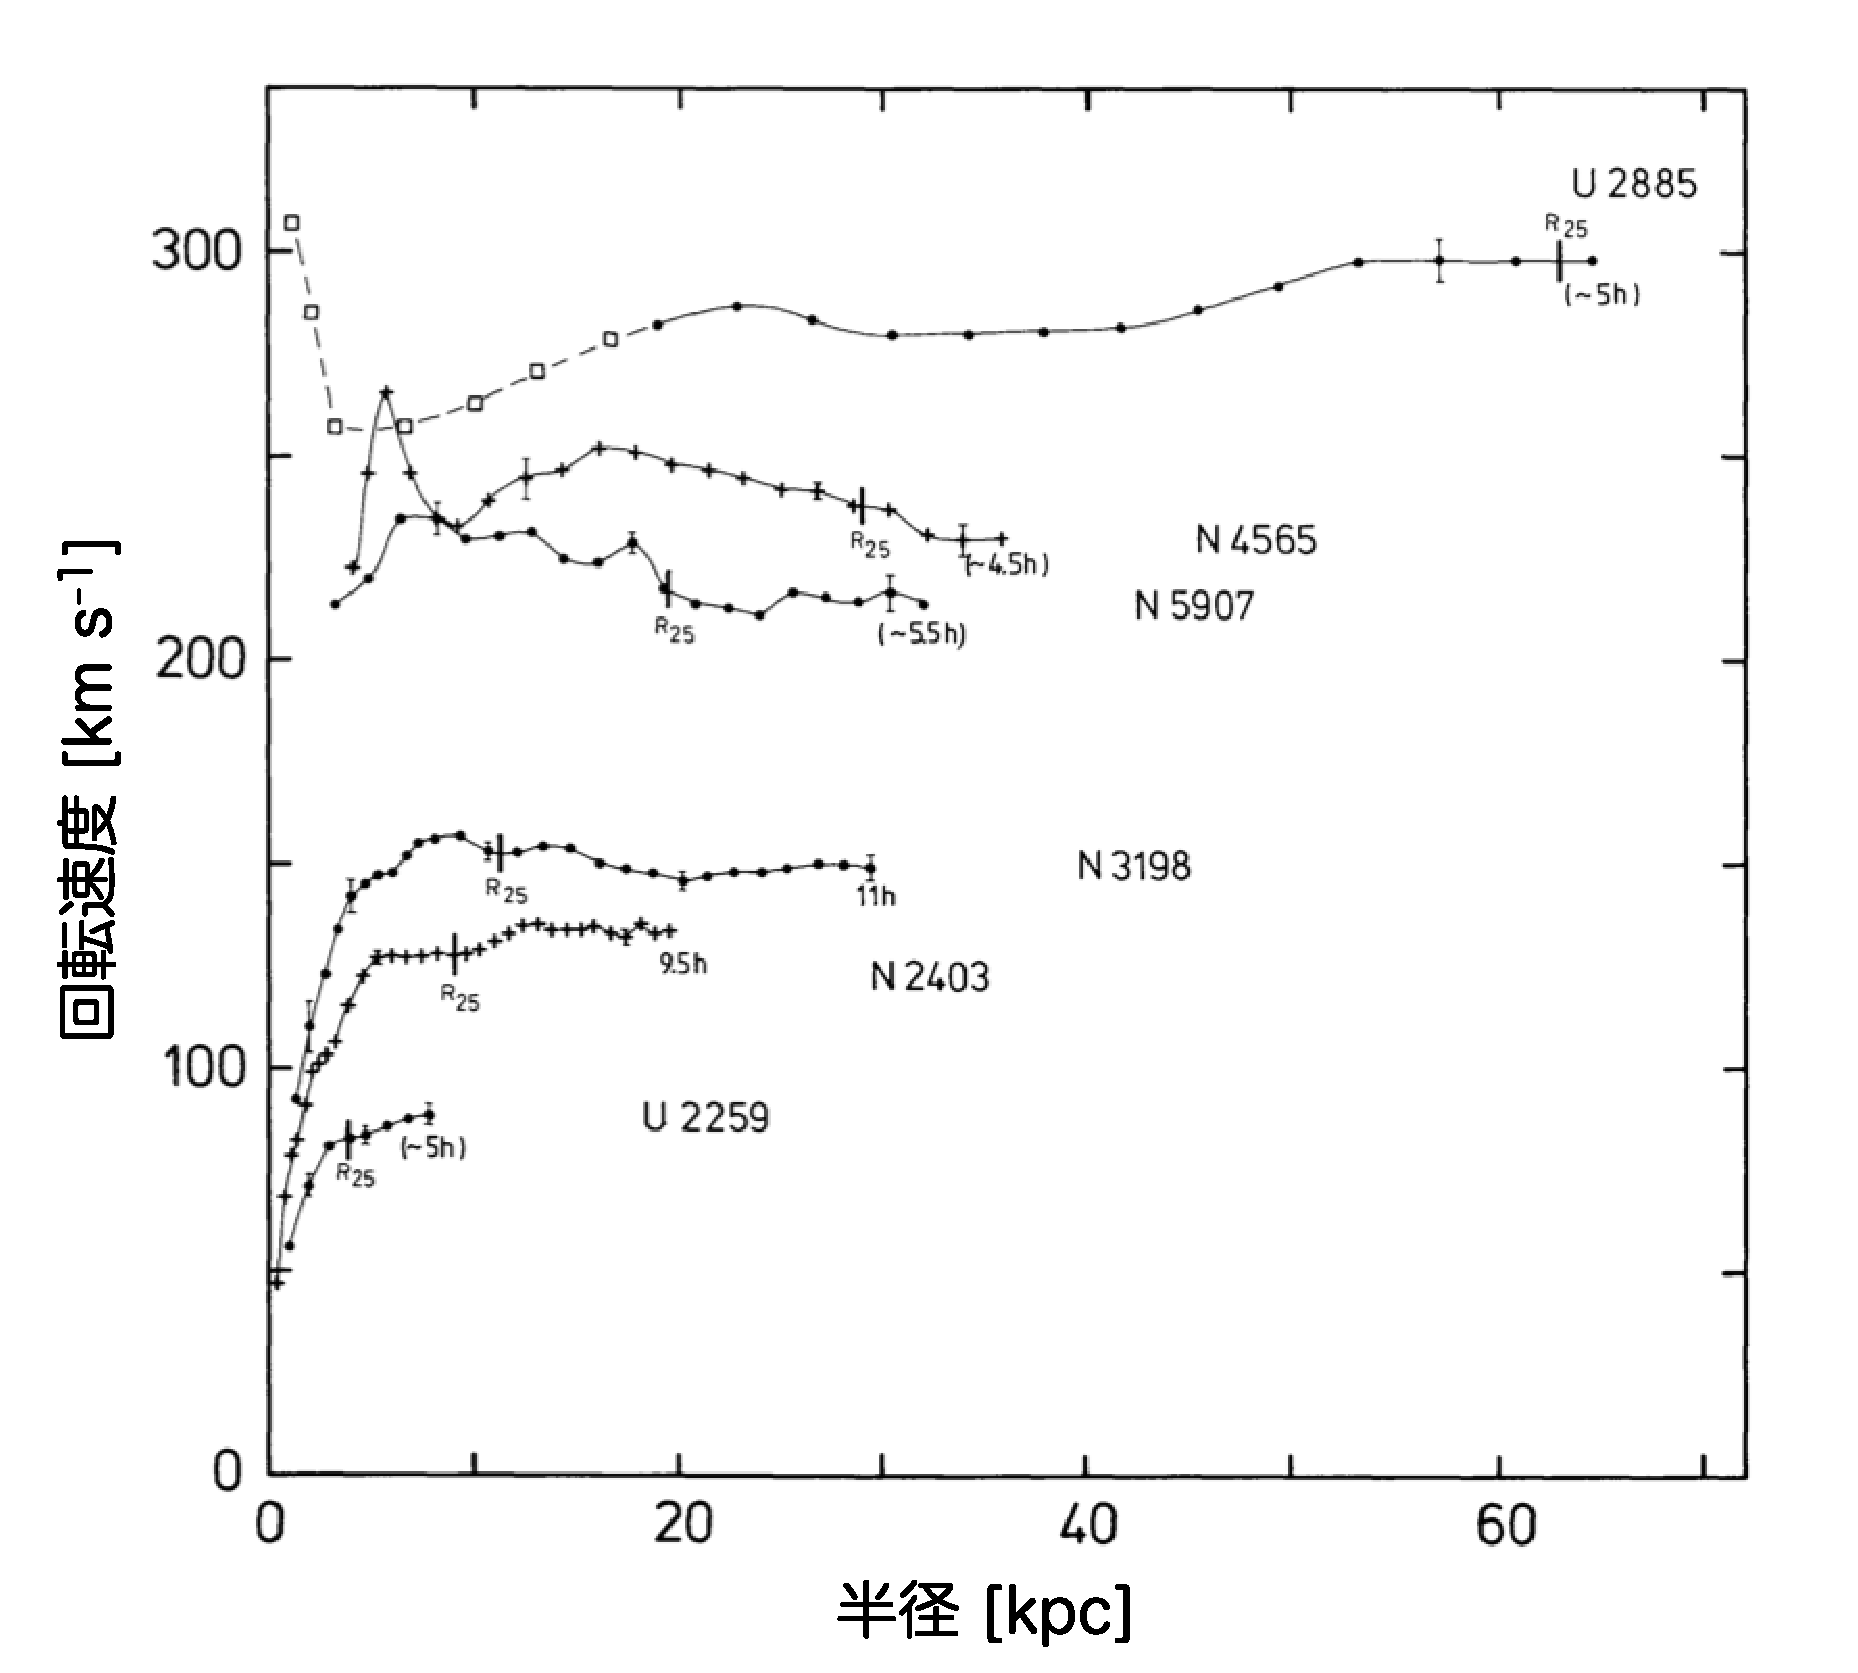
\includegraphics[width=14cm]{galaxy/Sancisi.eps}
\caption{様々な渦巻銀河の回転曲線(\citealt{1987IAUS..117...67S}を修正し転載)。$400\; \mbox{km s}^{-1}$を越える速い回転速度をもつ銀河は少ない。}\label{fig:deblok08}
\end{center}
\end{figure}
%%%

前述のように回転曲線は一般に半径に対してほぼ一定値をとることから、力学質量$M(r)$は半径に比例して増加することがわかる。また、回転速度が大きい銀河ほど総質量が大きくなることもわかる。
一方で、可視光や電波などの電磁波で観測される星やガス(H\,{\sc i}、分子)などの物質(バリオン)は銀河の外側にいくほど観測されにくい。これはバリオンの存在量が銀河の外側では少ないことを意味している。
%一方で、可視光や電波などの電磁波で観測される星やガス(H\,{\sc i}、分子)などの物質の分布は、 銀河の外側にいくほど暗く、存在量としては少なくなる。この違いは、
渦巻銀河の回転曲線から予想される力学質量と、観測から期待されるバリオン質量の不一致は、銀河の外側には観測されている物質以外に「見えない物質」が大量に存在していることを示唆している。この見えない物質をダークマターと呼ぶ。この、渦巻銀河の外側で見られる光学質量と力学質量の違いは銀河にダークマターが存在している一つの証拠となっている。


\subsubsection{タリー--フィッシャー関係}\label{sec:TF}

渦巻銀河の回転速度と真の明るさの間には``タリー--フィッシャー関係(TF関係)''と呼ばれる経験則がある\citep{1977A&A....54..661T}。
渦巻銀河の光度を$L$とすると、光度と回転速度($v_{\text{max}}$)の間には、$L\propto v_{\text{max}}^\alpha$($\alpha\approx4)$という関係が成り立ち、銀河における星成分とダークマター成分との関係を示す重要なスケーリング則である。
銀河の光度は銀河を構成する物質(主に星)の質量に比例するため、TF関係は銀河の星質量と回転速度の関係としても表すことができる。

TF関係は星質量が低い側において分散が大きくなることが知られている。これは、星質量が小さい渦巻銀河では星質量に対するガス質量の割合が無視できなくなるためである。そこで、星質量に加えガス質量も加えたバリオンの総質量($M_{\text{バリオン}} = M_* + M_{\text{ガス}}$)を用いることで、回転速度との相関が強くなる(分散が小さくなる)ことが示唆された\citep[e.g.,][]{2001ApJ...550..212B}。
この関係をバリオン-タリー--フィッシャー関係(BTF関係)という。
観測的には、近年行われている渦巻銀河のガス観測のサーベイデータを用い、BTF関係の検証が行われている\citep[e.g.,][]{2012AJ....143...40M}。

TF関係は渦巻銀河の距離を測定する指標としても使われている。
TF関係とH\,{\sc i}観測によって得られる銀河の回転速度から、銀河の真の明るさを見積ることができる。 一方、観測される銀河の明るさは距離に依存して変化する。そこで、銀河の真の明るさと観測される銀河の明るさの差を用いると、渦巻銀河までの距離を評価することができる。これまでは、H\,{\sc i}観測、星の分光観測それぞれで得られるTF関係から、渦巻銀河までの距離が調べられてきた。近年、特にBTF関係を用いることで高精度で距離決定ができることがわかってきた\citep[e.g.,][]{2001ApJ...550..212B}。しかし、観測的な星質量やガス質量の導出にはまだ多くの課題があり、その分、銀河までの距離決定にも不定性が生じうることに注意が必要である\citep[e.g.,][]{2014AJ....147..134Z}。

%%%%%%%%%%%%%%%%%%%%%%%%%%%%%%%%%%%%%%%%%%%%%%%%%%%%%%%%%%%%%%%%%%%%%%%%%%
\subsection{早期型銀河のHIガス}
\label{sec:早期型銀河の構造・運動・星種族}
%%%%%%%%%%%%%%%%%%%%%%%%%%%%%%%%%%%%%%%%%%%%%%%%%%%%%%%%%%%%%%%%%%%%%%%%%%


早期型銀河(楕円銀河・レンズ銀河)に関する従来の描像としては、バルジが卓越し(高いバルジ--ディスク比)、一様に古い星から構成されている、というものである。
しかし、バルジ--ディスク比がSc型渦巻銀河と同程度のものなど \citep{1951ApJ...113..413S,1970ApJ...160..831S,1976ApJ...206..883V}、早期型銀河にも形状の多様性があることが知られている。
また、大半の早期型銀河は、現在の星形成活動がほとんどないことが観測的に示されている \cite[e.g.,][]{1993PhDT.......172G,2000AJ....119.1645T,2005ApJ...619L.111Y,2007ApJS..173..619K,2010MNRAS.404.1775T}。
早期型銀河の運動状態や、構成している星に関しては、面分光観測により以下のようなことが明らかとなった;
多くの早期型銀河は回転しており、運動学的に冷たい系で \citep{2008MNRAS.390...93K}、回転している成分を構成している星はバルジよりも若く、metal-richである \citep{2010MNRAS.408...97K}。

$\mbox{ATLAS}^{\rm 3D}$は、260個の(morphologically-selectedな)早期型銀河に対する多波長での
サーベイ観測プロジェクトであり\footnote{http://www-astro.physics.ox.ac.uk/atlas3d/}、
上述の特徴を統計的に検証した。
その結果、サンプルの80~\%が軸対称な系で、fast rotating steller system
であること \citep{2011MNRAS.414.2923K, 2011MNRAS.414..888E}、大半が渦巻銀河から渦をとったような
系であること \citep{2011MNRAS.416.1680C}が示された。
また、多くの早期型銀河の星円盤はガスの冷却によって形成された、ということを示唆する結果が報告されており \citep{2011MNRAS.417..845K}、早期型銀河におけるガスの性質を理解することは、これらの銀河の構造の起源や、
星形成史を知る上で、非常に重要である。


\subsubsection{早期型銀河のH\,{\sc i}観測}


\subsubsection{単一鏡観測}

早期型銀河に対する単一鏡でのH\,{\sc i}観測は1960年代から活発に行われている。
単一鏡観測の空間分解能は干渉計観測に比べてよくないが、干渉計にある
missing flux (大きな空間スケールの構造に対する感度がないこと)の問題がないので、
銀河全体での情報 (H\,{\sc i}総質量、H\,{\sc i}スペクトルの線幅)を得るのに適している。
%初期の観測により、早期型銀河は、H\,{\sc i}ガス質量($M_{\rm HI}$)と$B$バンド光度($L_B$)の比($M_{\rm HI}/L_B$)が渦巻銀河よりも低いこと示された (e.g.,\cite{Gouguenheim+1969})。
1960年代の観測では、早期型銀河のH\,{\sc i}ガス質量($M_{\rm HI}$)と$B$バンド光度($L_B$)の比($M_{\rm HI}/L_B$)は、渦巻銀河よりも低いことが明らかになった \citep[e.g.,][]{1969A&A.....3..281G}。
その後、数100のサンプルに対して、典型的にH {\sc i}質量$M_\mathrm{HI}\sim (2-3)\times10^8$ $M_\odot$まで検出できるサーベイ観測が行われ、その結果、$\sim150$個の楕円銀河のうち15\%、$\sim300個$のレンズ銀河のうち25\%からH\,{\sc i}輝線が検出された \citep{1985AJ.....90..454K,1986AJ.....91...23W}。
またこれらの研究によれば、渦巻銀河で見られる$M_{\rm HI}-L_B$の相関関係は早期型銀河では見られず、これらの銀河のH\,{\sc i}ガスは銀河の外から来たものではないかと考えられている。

2000年に入ると、H\,{\sc i}での大規模な無バイアスな銀河サーベイのHIPASS \citep{2001MNRAS.322..486B}やALFALFA \citep{2005AJ....130.2598G}により、多くの早期型銀河からH\,{\sc i}輝線が検出された。
%特にALFALFAは、感度では$M_\mathrm{HI}<10^8$ $M_\odot$の銀河も検出でき、H\,{\sc i}輝線の検出率は、銀河の環境に強く依存することが示された;
特にALFALFAの感度は$M_\mathrm{HI}<10^8\; M_\odot$で、H\,{\sc i}輝線の検出率は、銀河の環境に強く依存することが示された;
乙女座銀河団に所属する早期型銀河からは数\% \citep{2007A&A...474..851D}、
乙女座銀河団外の早期型銀河からは40\%からH\,{\sc i}輝線が検出された \citep{2009A&A...498..407G}。
この結果は、H\,{\sc i}ガスは銀河団内部では容易にはぎとられる、という過去の研究 \citep[e.g.,][]{1983AJ.....88..881G}や、最近でも星形成をしているような早期型銀河は、銀河の密度が低い環境下にいる、という
観測事実\citep{2010MNRAS.404.1775T}とよく合う。


\subsubsection{干渉計観測}

1980年代には、干渉計を使った高分解能の観測により、早期型銀河におけるH\,{\sc i}ガスの分布や運動が詳細に研究され始めた。
早期型銀河のH\,{\sc i}ガスの分布に関しては、数$10$ kpcまで広がった低柱密度な円盤やリング構造や、ガス降着、はぎとり、銀河相互作用・合体を経験した(ている)かのような無秩序な構造など、非常に多岐に渡ることが明らかになった \citep[レビューとしては][]{1997ASPC..116..310V,2001ASPC..240..657H}。
また、これらの結果は、早期型銀河の質量獲得史を知る上で、H\,{\sc i}ガスが有力なトレーサーであることを示している。

\citet{2006MNRAS.371..157M}と\citet{2010MNRAS.409..500O}は、SAURONサンプル\footnote{
SAURON(Spectroscopic Areal Unit for Research on Optical Nebulae)は、William Herschel Telescopeの面分光装置であると同時に、楕円銀河・レンズ銀河・渦巻銀河のバルジの形成と進化を理解することを目的としたサイエンスプロジェクト \citep{2001MNRAS.326...23B}。
}
に含まれる早期型銀河を、典型的に$M_\mathrm{HI}\sim (2-3)\times10^6$ $M_\odot$まで検出できる感度で観測し、環境効果、H\,{\sc i}ガス分布、その運動状態を詳細に調べた。
%Morganti et al. (2006)・Oosterloo et al. (2010)は、それぞれ12・33天体を観測、9・15天体からH\,{\sc i}を検出し、環境効果、H\,{\sc i}ガス分布、その運動状態を詳細に調べた。
その結果、乙女座銀河団に所属する/しない早期型銀河からは10\%、$2/3$の検出率でH\,{\sc i}輝線を検出した。
H\,{\sc i}輝線が検出された銀河のうち、半数は円盤・リング構造を持ち、それらは$1\sim$ 数10 kpcの広がりを持つことが明らかになった。
また、1) 安定したH\,{\sc i}の構造を持つすべての早期型銀河は、1有効半径($R_{\rm e}$)内に電離ガスが存在し、H\,{\sc i}ガスと電離ガスは同じ運動をしていることや、2) $1R_{\rm e}$以内にH\,{\sc i}ガスが存在するすべての早期型銀河は、一酸化炭素分子(CO)輝線と電波連続波が検出されていることなど、最近の星形成を示唆する結果が得られている。

%\subsubsection{H\,{\sc i} survey toward ATLAS$^{\rm 3D}$ sample}
\subsubsection{ATLAS$^{\rm 3D}$サンプルに対するH\,{\sc i}サーベイ}

\ref{sec:早期型銀河の構造・運動・星種族}章の冒頭で紹介したように、ATLAS$^{\rm 3D}$は早期型銀河に特化した、大規模な多波長サーベイである。
このサーベイは、$42$ Mpc以内に存在する、$M_{\rm K}=-21.5$よりも明るい、260個の早期型銀河が対象となっており、そのうち、H\,{\sc i}が観測されたのは、Westerbork Synthesis Radio Telescope(WSRT)で観測可能な銀河170天体である \citep{2012MNRAS.422.1835S}。
その結果、$5\times10^6-5\times10^7$ $M_\odot$の感度を達成し、53天体からH\,{\sc i}輝線を検出した。
これらの銀河の解析から、主に以下の5点を明らかにした。

\begin{description}

\item[(i) H\,{\sc i}形態] リング・円盤などの構造(H\,{\sc i}輝線が検出された53天体のうち$\sim64$ \%)や、潮汐力、もしくはガス降着によるtail構造を含む無秩序な構造($\sim26$ \%)、また銀河全体に散らばったクラウド構造($\sim9$ \%)など多岐にわたる。
リング・円盤構造を持つ早期型銀河を、その広がりの大きさで2つに分けると(境界半径:$3.5\times R_{\rm e}$)、以下のような違いがある;
大きいH\,{\sc i}円盤(数10 kpc)は、$M_{\rm HI}\sim5\times10^9$ $M_\odot$で、半数は星成分とは
異なる運動をしており、
小さなH\,{\sc i}円盤は、$M_{\rm HI}<10^8$ $M_\odot$で、星成分と同じ運動をしている。

\item[(ii) 星形成] $\sim1R_{\rm e}$以内にH\,{\sc i}ガスが存在する銀河のうち$70$ \%は、星形成をしており(銀河の中心領域は分子ガスが支配的)、$\sim1R_{\rm e}$以内にH\,{\sc i}ガスが存在しない銀河と比べて、その発生頻度は5倍である。
また、小さなH\,{\sc i}円盤がある銀河のH\,{\sc i}ガスからH$_2$ガスへの変換効率は、渦巻銀河と同程度である。

\item[(iii) H\,{\sc i}質量関数] Schechter関数でフィットすると、折れ曲がりが起こる質量は$M^\ast\sim2\times10^9$ $M_\odot$、低質量側の傾きは$\alpha\sim-0.7$である\footnote{H\,{\sc i}で観測されるすべての銀河の種族が単一のSchechter関数でフィットできるわけではない。}。

\item[(iv) 渦巻銀河との比較] 全体的に渦巻銀河と比べると早期型銀河のH\,{\sc i}質量は
小さいが、中には渦巻銀河と同程度のH\,{\sc i}質量を持つような早期型銀河もいる。
渦巻銀河の明るい星円盤で見られるようなH\,{\sc i}柱密度の高い成分は、早期型銀河にはない。

\item[(v) 環境効果] 乙女座銀河団に所属する早期型銀河のうち$\sim10$ \%、所属しない早期型銀河のうち$\sim40$ \%から輝線を検出し、銀河団に所属しない早期型銀河にはH\,{\sc i}ガスが存在する一般性を示した。
周囲の銀河の密度が高いほど、$M_{\rm HI}$、$M_{\rm HI}/L_K$比は連続的に小さくなり、最もガスリッチな早期型銀河は周囲の銀河密度が最も低いような環境に存在する。
そのような環境下では、星形成の兆候が見られる割合が高い。
乙女座銀河団の中心に存在する早期型銀河のH\,{\sc i}ガス質量は最も少ない。
一方、銀河団の外側に存在する早期型銀河は、多くのH\,{\sc i}ガスを含んでおり、少なくとも、
それらの一部は、%%銀河群を形成した後、(銀河群に言及するのは必要??)
最近銀河団に落ちてきたと考えられる。
H\,{\sc i}の形態と銀河密度の間には関係があり、銀河密度が低い環境には、大きな円盤・リングを持つものが多く、乱れたH\,{\sc i}形態を持つ銀河はrich groupの典型的な銀河密度環境下に多く存在する。
このことは、早期型銀河の進化には、銀河--銀河団スケールで起こるプロセスが重要であることを示唆している。
\end{description}


%%%%%%%%%%%%%%%%%%%%%%%%%%%%%%%%%%%%%%%%%%%%%%%%%%%%%%%%%%%%%%%%%%%%%%%%%%
\subsection{矮小銀河のHIガス}
\label{sec:矮小銀河のHIガス}
%%%%%%%%%%%%%%%%%%%%%%%%%%%%%%%%%%%%%%%%%%%%%%%%%%%%%%%%%%%%%%%%%%%%%%%%%%

矮小銀河は低質量ダークハロー(DH)に付随していると考えられており、$\Lambda$CDMモデルにおいては、このような低質量なDHから初代星が生まれてきたと考えられている \citep{2006ApJ...652....6Y,2008Sci...321..669Y}。
%しかし、近傍に存在する矮小銀河でさえ、その銀河スケールの星形成は未だによくわかっていない。
ガスリッチ、低質量、低金属量、低表面輝度な天体である矮小銀河の星形成の理解は、宇宙初期の星形成の理解にも繋がる重要なステップである。
また、矮小銀河は大きな銀河のbuilding blockであると考えられており、銀河進化の解明のためにも、矮小銀河の性質を明らかにすることは極めて重要な課題である。
大規模な銀河サーベイは、主に可視光や近赤外線で野心的に行われているが、これらのサーベイでは比較的明るく星質量が大きい天体に偏りがちである。
一方近年の大規模・高感度なH\,{\sc i}サーベイにより、多くのガスリッチな矮小銀河が見つかった。
以下では、矮小銀河に特化したH\,{\sc i}サーベイについて紹介する。


\subsubsection{矮小銀河に対するHIサーベイ}

過去数10年は、主に、H\,{\sc i}質量が$10^8$ $M_\odot$よりも大きい矮小銀河の運動や星種族が詳細に調べられてきた。例えば、
大規模な無バイアス銀河H {\sc i}サーベイ、ALFALFA \citep{2005AJ....130.2598G} により、H\,{\sc i}質量の小さな銀河($<10^8$ $M_\odot$)が数百個観測され、低質量側までを含む、統計的に信頼できるH\,{\sc i}の質量関数が初めて示された\citep{2010ApJ...723.1359M}。
以下では、中でも質量の小さい矮小銀河に対する代表的な4つのサーベイ(FIGGS、LITTLE THINGS、VLA-ANGST、SHIELD)の紹介を行う。

FIGGS \citep{2008MNRAS.386.1667B}、LITTLE THINGS \citep{2012AJ....144..134H}、VLA-ANGST \citep{2012AJ....144..123O}は、比較的質量の低い矮小銀河を対象としており、それぞれのサーベイのサンプルのH\,{\sc i}質量の中央値は、それぞれ$8.5\times10^7$ $M_\odot$、$2.7\times10^7$ $M_\odot$、$2.3\times10^7$ $M_\odot$である。
SHIELD \citep{2011ApJ...739L..22C}は特に質量が小さいサンプルを対象としており、H\,{\sc i}質量が$10^6-10^7$ $M_\odot$の銀河サーベイである。
なお、前述した3つのサーベイにも、$10^7$ $M_\odot$より低いH\,{\sc i}質量の銀河が合計21個含まれている (4個、LITTLE THINGS; 8個、FIGSS、9個、VLA-ANGST)。
上述したサーベイにおけるサイエンステーマは、主に以下の4点である。

\subsubsection{(i) ガスリッチな矮小銀河の存在 (SHIELD)}

%$\Lambda$-CDMの枠組みにおいて、ガスリッチな矮小銀河の存在は、興味深い難題の一つである。
%質量の小さな系は、以下の4つの理由からgas poorになることが予想されている。
質量の小さな系は、以下の4つの理由からガスが少なくなると予想されている。

\noindent
{\bf 1) 動圧(ram pressure)によるはぎ取り}。
矮小銀河が、大きな銀河や銀河団のビリアル半径内にいれば、それらのコロナルガス
%coronal gas
によって、星間物質(interstellar medium: ISM)がはぎ取られてしまう \citep[e.g.,][]{2002MNRAS.334..673L,2003AJ....125.1926G}。

\noindent
{\bf 2) 星形成による銀河風でのガスの喪失}。
数値シミュレーションによれば、H\,{\sc i}質量が$10^7\; M_\odot$よりも小さい場合、爆発的星形成に起因する強い銀河風(galactic superwind)によって質量損失されやすいことが予想されており \citep[e.g.,][]{1999ApJ...513..142M,2000MNRAS.313..291F}、このシナリオを支持する観測結果も存在する \citep[e.g.,][]{2002ApJ...574..663M,2005MNRAS.358.1453O}。

\noindent
{\bf 3) 銀河外からのUV輻射による降着ガス、ガス冷却の抑制}。
halo質量が小さいほど、銀河外からのUV輻射の影響を受けやすい \citep{1986MNRAS.218P..25R,1992MNRAS.255..346B,2002MNRAS.333..156B,2006MNRAS.371..401H}。

\noindent
{\bf 4) hot intergalactic medium (IGM) によるガスの蒸発。}
Hubble時間以内に、小さく、シールドされていないcold gasは、hot IGMにより蒸発されてしまう \citep{2002MNRAS.333..156B}。
上記4点から、質量が小さな系はガスが少なくなると予想されているのにも関わらず、観測では多くのガスリッチな矮小銀河が見つかっている。
中にはH\,{\sc i}質量が$\sim10^5$ $M_\odot$の銀河も報告されている \citep[Leo T: ][]{2007ApJ...656L..13I}。

ガスリッチな矮小銀河の性質の理解は、halo質量の小さな系に働く上述のガス欠乏メカニズムの制限に繋がる。
また、低質量矮小銀河の観測は、天の川銀河における極めて低質量な伴銀河 \citep[e.g., Willman 1, H\,{\sc i}質量 $\sim5\times 10^5$ $M_\odot$,][]{2005ApJ...626L..85W,2007MNRAS.380..281M} と、研究の進んでいる質量の大きな矮小銀河の間にある観測のギャップを埋めることができる。
なおこの範囲は、バリオン含有量が宇宙の平均値 ($0.16$) から$<0.01$になるhaloの質量範囲を含んでいる \citep{2006MNRAS.371..401H,2010ApJ...708L..14M}。


\subsubsection{(ii) 極端な環境下でのクラウド・星形成 (VLA-ANGST, LITTLE THINGS, FIGGS)}


渦巻銀河における渦状腕上や、銀河の合体衝突では、ガスが圧縮され星形成が誘発されるが、そのような外からの摂動がない場所での星形成を調べる上で、gas-richな矮小銀河は最適な研究対象である。


%\subsubsection{(iii) 矮小銀河のTully-Fischer、Baryonic Tully-Fischer関係}
\subsubsection{(iii) 矮小銀河のタリー・フィッシャー、バリオン タリー・フィッシャー関係}

%Tully-Fischer (TF) 関係は、渦巻銀河の銀河の明るさ(星質量)と、銀河全体でのH\,{\sc i}輝線の線幅($\sim$回転速度、DM質量)の間に見つかった経験則である。
%これは、銀河における星成分とDM成分との関係を示す重要なスケーリング則である。
矮小銀河は渦巻銀河のTF関係に乗らないが、銀河の明るさの代わりに、バリオン質量を使った、BTF関係には従うことが報告されている \citep{2000ApJ...533L..99M,2005ApJ...632..859M}。


\subsubsection{(iv) ダークマター分布}

階層的銀河形成の宇宙論的シミュレーションは、
%DMHの密度プロファイルが普遍的なカスプありの形状になることを予言している
DHの中心部がカスプ状の密度プロファイルとなることを予言している \citep[e.g.,][]{2004MNRAS.349.1039N}。
その予言を支持する観測がある一方で \citep[e.g.,][]{2001MNRAS.325.1017V,2005ApJ...634..227D}、矮小銀河において、DMHは密度一定の中心コアを持っているという観測結果も存在している \citep[e.g.,][]{2003MNRAS.340..657D,2003MNRAS.340...12W}。

一般に、観測から求める銀河におけるダークマターの分布には、星の質量-光度関係
%M/L
に起因する大きな不定性が残ってしまう。
しかし矮小銀河は星からの寄与が少ないため、ガスの運動からダークマターの密度プロファイルを正確に調べることができる。故に、矮小銀河のH {\sc i}サーベイは、ダークマター分布の普遍性について調べるのに
適している。


%%%%%%%%%%%%%%%%%%%%%%%%%%%%%%%%%%%%%%%%%%%%%%%%%%%%%%%%%%%%%%%%%%%%%%%%%%
\subsection{様々な種族にまたがるサーベイ(銀河進化の統計的、統一的理解に向けて)}
\label{sec:様々な種族にまたがるサーベイ}
%%%%%%%%%%%%%%%%%%%%%%%%%%%%%%%%%%%%%%%%%%%%%%%%%%%%%%%%%%%%%%%%%%%%%%%%%%

銀河進化を理解する上で、銀河の各種族ごとの詳細な性質を調べることも重要であるが、銀河全体としての性質を調べることも合わせて
重要である。これまで、渦巻銀河(\ref{sec:spiral}章)・早期型(\ref{sec:早期型銀河の構造・運動・星種族}章)・矮小銀河(\ref{sec:矮小銀河のHIガス}章)に対するH\,{\sc i}観測について個別に紹介してきたが、
\ref{sec:様々な種族にまたがるサーベイ}章前半では、$z \sim 0$における銀河の統計的性質を調べることに重きを置いた大規模なサーベイプロジェクトであるGASSプロジェクトを
紹介する。また、\ref{sec:様々な種族にまたがるサーベイ}章の後半では、SKAのターゲットとなりうる中間赤方偏移帯($0.1<z<1.0$)の銀河に対する2つのサーベイ、BUDHIES、
CHILESプロジェクトを紹介する。

\subsubsection{GALEX Arecibo SDSS Survey (GASS)}

Sloan Digital Sky Survey \citep[SDSS,][]{2000AJ....120.1579Y}などの可視光での大規模な銀河サーベイにより、星質量 vs $u-r$カラープロット上で、銀河はbimodal分布することが明らかになった \citep[e.g.,][]{2001AJ....122.1861S}; 
青く、星を活発に形成している``blue cloud''、現在は星形成をしていないような``red sequence''、両者の境界質量は$\sim3\times10^{10}$ $M_\odot$。
GALEX Arecibo SDSS Survey \citep[GASS,][]{2010MNRAS.403..683C}は、この二つの種族間を遷移しているような銀河(``遷移銀河''、ガス降着している銀河/星形成がquenchしている銀河)を特定し、その割合を定量化することを主な目的としている。
観測は、世界で最も大きい電波望遠鏡である、アレシボ観測所の305~m鏡を使い、2008年3月から2012年7月の間に行われた。
サンプル銀河は、SDSSで分光観測され、Galaxy Evolution Explorer \citep[GALEX,][]{2005ApJ...619L...1M}で撮像されている銀河の中から抽出された。
条件は、赤方偏移と星質量のみで、それぞれ$0.025<z<0.05$、$10<\log{M_\star/M_\odot}<11.5$である。
星質量の範囲は、青い/赤い銀河間の遷移質量である$\sim3\times10^{10}\; M_\odot$を含むように選ばれている。
観測は、H\,{\sc i}輝線が検出されるか、もしくはH\,{\sc i}ガスの割合が$1.5-5\; \%$に到達するまで行われる。

%およそ4年間にわたる観測により、8編の論文が出版されている。
以下ではそれらの主な7つの結果を紹介する。

\paragraph{(i) HIガスの割合 \citep{2010MNRAS.403..683C,2012MNRAS.420.1959C}}

H\,{\sc i}ガスの割合($=M_{\rm HI}/M_\star$)は、星質量($M_\star$)、星質量の表面密度($\mu_\star$)、NUV$-r$カラーに反比例して減少するのに対し、バルジ--ディスク比($\sim$中心集中度、$C=R_{\rm 90}/R_{\rm 50}$、$R_{\rm 90}, \; R_{\rm 50}$は$r$バンドの光の90, 50~\%を含んでる半径)にはほとんど依存しない。
$M_{\rm HI}/M_\star$が高い銀河(ガスリッチ)の割合は、$M_\star$が大きくなるほど連続的に下がるのに対し、$\mu_\star$に対しては不連続に変化し、$\mu_\star>10^{8.5}$ $M_\odot$ kpc$^{-2}$で急激に下がる。

$M_{\rm HI}/M_\star\mbox{--}\mu_\star\mbox{--} ({\rm NUV}-r)$の間にはスケーリング則が成り立ち、``遷移銀河''は、このスケーリング則から外れると考えられる。
$M_{\rm HI}/M_\star$が$50$\%であるような早期型銀河GASS 3505(おそらく赤い種族から青い種族へ)や、$2$\%程度しかない円盤銀河GASS 7050(青い種族から赤い種族へ)は、このスケーリング則から外れたところに分布する。


\paragraph{(ii) 星形成効率 \citep{2010MNRAS.408..919S}}

$M_\star$、$\mu_\star$、NUV$-r$、$C$に反比例するspecific SFR ($\mbox{sSFR} = \mbox{SFR}/M_\star$)と違い、星形成効率($=\mbox{SFR}/M_{\rm HI}$)の平均は全サンプルを通して、これらの量に対してほぼ一定の値を持つ ($\mbox{SFE}=10^{-9.5}\;\mbox{yr}^{-1}$、もしくはガス消費のタイムスケールでは3~Gyrに相当)。
このことは、ガス供給を制御する外部過程や星形成フィードバックが、比較的質量の大きな銀河における星形成の調整機構として重要であることを示唆している。
しかし個々の銀河を見ると、平均よりもSFEが高い銀河と低い銀河が同じ割合ずつ存在しており、これらの銀河は、sSFRを近い将来に変化させる可能性を持つ``遷移銀河''の候補である。


\paragraph{(iii) 銀河円盤の``inside-out formation'' \citep{2011MNRAS.412.1081W}}

H\,{\sc i}ガスが豊富な銀河とそうでない銀河を比較すると、H\,{\sc i}ガスが豊富な銀河ほど、青く、より活発に星形成をしていることが明らかになった。
また、H\,{\sc i}ガスの割合が高い銀河ほど、銀河円盤の外側ほど青く、活発に星形成している。
この結果は、円盤銀河は内側から形成されたという``inside-out''成長シナリオを支持する。
一方で、H\,{\sc i}ガスの割合と、銀河の軸対称さの間に関係がないことは、ガスが銀河外縁部に滑らかに降着していきていることを示唆している。

\paragraph{(iv) バリオン質量--速度--サイズ関係 \citep{2012A&A...544A..65C}}

H\,{\sc i}が検出されたかどうかに限らず、すべてのサンプルを使うと、
%baryonic Faber-Jackson (BFJ)関係(バリオンの質量と星の速度分散との関係)は、baryonic Tully-Fisher (BTF)関係よりも分散が小さくなる。
バリオン フェーバー--ジャクソン(BFJ)関係(バリオンの質量と星の速度分散との関係)は、BTF関係よりも分散が小さくなる。
また、BFJ関係は、BTF関係で問題になる銀河の傾き(inclination)の影響は受けない。
円盤が卓越したガスリッチ銀河は、回転楕円体(楕円銀河や、バルジ)で定義されるBFJ関係から系統的にずれるが、星の速度分散を銀河の中心集中度を使って補正すると、同じ関係に乗る。また、この一般化されたBFJ関係は、銀河の形態、inclination、ガスの量に関係なく存在し、分散は0.1~dex以下である。円盤の速度-サイズ関係は、回転楕円体のものからはずれるが、上述の方法で星の速度分散を補正すると同じ関係上に乗る。

これらの結果は、銀河のglobalなダークマターとバリオン成分の間には基本的な関係があり、これは銀河の形態に関係なく存在していることを示している。


\paragraph{(v) 銀河外縁部での金属汚染 \citep{2012ApJ...745...66M}}

GASS銀河の平均的な金属量の動径分布は$R_{\rm 90}$まで平坦であるが、比較的質量が小さい($\log{(M_\star)}<10.2$)、中心集中度が低い、星質量の表面密度が低い、銀河は半径が大きくなるほど金属量が下がる傾向が見られる。
しかし、$R_{\rm 90}$よりも外側では、サンプル銀河のうち$10$\%が急激に金属量が下がる。
この金属量の降下の度合いは、銀河におけるH\,{\sc i}ガスの割合と関係しており、H\,{\sc i}ガスの割合が大きい銀河ほど、銀河の外側で金属量が急激に下がる。
また、銀河外縁部で急激に金属量が下がる銀河は、活発に銀河円盤を形成しており、このような銀河は、星質量を2倍にするタイムスケールが一般的なGASS銀河の1/3程度である。
局所的な星質量密度と金属量は相関しており、これは、全サンプルで成り立つ。
銀河外縁部における激しい星形成は、ガス降着、もしくは、星円盤よりも外側にあった低金属量なガスが動径方向に輸送される事によって引き起こされている可能性がある。


\paragraph{(vi) 異なる星質量ごとでのH I質量関数 \citep{2013ApJ...776...74L}}

H\,{\sc i}質量関数は、宇宙論的シミュレーションに制限を与え、銀河におけるH\,{\sc i}ガス量の観測的予想のテストに使うことができ、平均的な傾向からずれている銀河を特定することができる。

GASSサーベイの結果から求まるH\,{\sc i}質量関数は、Schechter関数で表現できるような形をしている。
近傍宇宙のH\,{\sc i}密度の41~\%は質量の大きな銀河によることと、
Schechter関数のパラメータは星質量の違いではあまり変わらないことが明らかになった。
H\,{\sc i}ガスの割合が1~\%以上ある銀河の割合と星質量の間の関係は、
銀河形成・進化モデルに対する強い制限となる。Schechter関数のパラメータはSFRに依存している。


\paragraph{(vii) 環境効果 \citep{2013MNRAS.436...34C}}

銀河群に典型的な、質量が$10^{13\mbox{--}14}\; M_\odot$程度あるhalo内に存在する銀河は、
銀河の密度が低い環境下にいる同じ星質量の銀河に比べて、少なくとも$0.4$ dexはH\,{\sc i}が少ない。
銀河群におけるガスの抑制に効く過程は、これらの系で観測される星形成のquenchingを引き起こしていると考えられる。
この結果は、銀河進化において銀河群という環境の重要性を示しており、準解析的銀河形成モデルにおいて、銀河群での冷たいISMのはぎ取りを入れる必要性を示唆している。


\subsubsection{中間赤方偏移($0.1<z<1.0$)}

COSMOS H\,{\sc i} Large Extragalactic Survey \citep[CHILES,][]{2013ApJ...770L..29F}とBlind, Ultra-Deep H\,{\sc i} Environmental Survey \citep[BUDHIES,][]{2007ApJ...668L...9V}は、積分時間が1000時間程度にも及ぶ観測をして、$z\sim0.2$の銀河からH\,{\sc i}を検出した。
%しかし、今のところ$z=0.2$よりも遠方の銀河からH\,{\sc i}を検出するには、可視光のデータカタログから位置と赤方偏移の情報を使って、スタッキングすることで成功を収めている。
しかし今のところ、$z=0.2$よりも遠方の銀河からのH\,{\sc i}輝線の検出は、可視光の観測から求まっている位置と赤方偏移を使って、スタッキングすることで成功を収めている。
下で、中間赤方偏移のH {\sc i}観測に関する重要なものをいくつか挙げる。

\paragraph{(i) BUDHIESサーベイ \citep{2007ApJ...668L...9V}}

性能向上したWesterborkの受信機システムを使い、%Blind, Ultra-Deep H\,{\sc i} Environmental Survey (BUDHIES)
BUDHIESは、$z=0.187$のAbell~2192 (A~2192)、$z=0.206$のAbell~963 (A~963)という2つの銀河団の観測を行った。
A~963は、質量が大きく、重力レンズ効果があり、X線でも明るい、Butcher--Oemler銀河団で、特徴としては、他の銀河団と違って、銀河団の中心領域に存在する青い銀河の割合が極めて高い点が挙げられる。
BUDHIESの主なサイエンスゴールの一つは、これらの中心領域の青い銀河と、銀河団の外側にいる、また、この銀河団の周辺の孤立した青い銀河の関係を、H\,{\sc i}ガス量という観点から明らかにすることである。
一方で、A~2192は低質量な銀河団で、A~963の比較対象として観測される。

2つの銀河団で同じ質量感度($2\times10^9$ $M_\odot$)が達成できるように、A~2192には$78\times12$時間、A~963には$117\times$12時間かけてデータが取得された。
その結果、合計39個の銀河からH\,{\sc i}輝線が検出された。
パイロットサーベイにおいて、A~963中心領域の青い銀河からは、スタッキングをしてもH\,{\sc i}輝線は検出されなかったが、似たような光度、カラーのfield銀河からはH\,{\sc i}が検出された \citep{2007ApJ...668L...9V}。
銀河団の内部や、外部のsubstructureの銀河におけるH\,{\sc i}ガス量も調べられている \citep{2013MNRAS.431.2111J}。
また、$z\sim0.2$でのTF関係も調査されている。

\paragraph{(ii) CHILESサーベイ \citep{2013ApJ...770L..29F}}

%COSMOS H\,{\sc i} Laege Extragalactic Survey (CHILES)
CHILESは現在も進められているVLAを使った1000時間のプログラムである。
装置の性能向上により、$z=0-0.51$に存在する銀河のH\,{\sc i}輝線検出が可能となっている。
これにより、これまでのH\,{\sc i}観測が行われている銀河までのlook-back timeが二倍になる。
このプログラムはVLAのB配列で、COSMOS領域の中心1点を観測する。
CHILESによって、最も遠くの天の川銀河のような銀河や、$4\times10^5$ Mpc$^3$の領域の300以上のH\,{\sc i}-rich天体のH\,{\sc i}ガス分布が明らかにされると期待されている。
この領域の、低・中間・高赤方偏移には宇宙の大規模構造が存在しており、COSMOS領域は多波長のデータが揃っているため、銀河の性質、環境、時間の関数として銀河進化を調べることができる。
CHILESは、宇宙の星形成率密度が低下している時代の、銀河におけるH\,{\sc i}ガス量、その進化、形態を調べることができる最初のサーベイである。

すでに50時間の観測で、$34'\times34'$の領域の$z=0\mbox{--}0.193$に存在する銀河のうち、33天体からH\,{\sc i}輝線を検出した。
そのうち、3天体はこれまで分光による赤方偏移の情報がない天体であった。
33天体のうち、最も遠い銀河は$z=0.176$で、H\,{\sc i}質量は$8\times10^9\; M_\odot$である。
$z=0.12-0.13$間に存在する``wall''に存在する80個の銀河のスペクトルをスタッキングしたところ、$1.8\times10^9\;  M_\odot$に相当するH {\sc i}輝線が検出された。
これらの初期成果は\citet{2013ApJ...770L..29F}にまとめられており、カタログは現在準備中である (Hess et al. in prep.)。

\paragraph{(iii) スタッキングによる結果}

上述したサーベイなどにより、$z\sim0.1$より遠方の個々の銀河からH\,{\sc i}輝線が検出され始めているが、幅広い宇宙年齢における銀河のH\,{\sc i}ガスの量は、スタッキング解析によって明かになることが予想される。
今やスタッキングは、一つのサーベイにおいて、個々の天体からは信号が検出されなかったような種族の統計的な性質に制限を加える一般的な手段となった。
そしてH\,{\sc i}データを含め、様々な天文データに適用されてきた。
この手法を適用するためには、独立な方法で銀河の座標と赤方偏移を調べる必要がある。
例えば、可視光サーベイで見つかった、赤方偏移も既知の銀河のH\,{\sc i}データをスタッキングする場合、H\,{\sc i}のcubeデータの中から、該当する場所のデータを抽出し、天体の赤方偏移に応じて周波数軸をずらして、一般的には適切に重みを付けて足し合わせられる。
足し合わせるデータの数$N$に応じて、雑音は理論上は$1/\sqrt{N}$で下がるので、個々の天体からは検出できない微弱なH\,{\sc i}輝線の検出を可能にする。

星形成率密度が低下してきている中間赤方偏移帯における、H\,{\sc i}のcosmic density, $\Omega_{\rm HI}$を決定することは極めて重要である。
%過去10年の間、H\,{\sc i}ガスの進化はスタッキング解析によって調べられてきた。
\citet{2007MNRAS.376.1357L}は、Giant Metrewave Radio Telescope (GMRT)を使い、$z\sim0.24$の星形成銀河のH\,{\sc i}量を、\citet{2013MNRAS.435.2693R}はWSRTを使い、$z\sim0.1$と$z\sim0.2$の銀河のH\,{\sc i}量を調べた。
スタッキング解析の結果、彼らはlook-back timeが$2-4$ Gyrにおける$\Omega_{\rm HI}$に制限を加えることに成功した。
これらの研究は遠方のDamped Ly$\alpha$天体に対するH\,{\sc i}の吸収線観測と、近傍銀河に対するH\,{\sc i}での無バイアスサーベイの橋渡しをする重要な研究である。


銀河環境や時間の関数として、ガス、星形成、その他の銀河の性質の間の関係を調べる上で、スタッキングは非常に強力な手法である。
可視光データから抽出された、およそ5000個のALFALFA銀河のスタッキング解析により、ガスの割合と銀河の構造や星形成の性質を結びつけるスケーリング則 \citep{2011MNRAS.411..993F} や、銀河内のガスに与える環境効果 \citep{2012MNRAS.427.2841F} が明らかになった。
%これらの研究は大きな統計が必要である上に、ガス量が少ない天体のH\,{\sc i}の情報を得る必要があるため、個々の銀河から輝線を検出するよりも、スタッキング解析の方が好ましい。
環境効果に関しては、$z\sim0.2$ \citep{2007ApJ...668L...9V} や$z=0.37$ \citep{2009MNRAS.399.1447L}でも調べられている。



%%%%%%%%%%%%%%%%%%%%%%%%%%%%%%%%%%%%%%%%%%%%%%%%%%%%%%%%%%%%%%%%%%%%%%%%%%
\subsection{高赤方偏移へ: 水素原子吸収線系による銀河進化の解明}\label{sec:DLA}
%%%%%%%%%%%%%%%%%%%%%%%%%%%%%%%%%%%%%%%%%%%%%%%%%%%%%%%%%%%%%%%%%%%%%%%%%%

銀河の宇宙における分布は、大規模構造という宇宙最大の構造を形作っており、銀河の形成・進化は、宇宙構造形成の根本的な問題である。しかしながら、観測的に遠方(高赤方偏移)の銀河を観測することは、常に、明るいものしか見えない(サンプルが明るいものに偏る)という問題がある。つまり、星がまだあまり形成されていない、まだ星の材料である星間ガスが豊富な「原始的な銀河」は、暗すぎてサンプルから漏れる。星間ガスが豊富な銀河を探査する方法として現在世界的に行われているのが、クエーサーを背景光にしてその視線方向にある水素ライマンアルファ(Ly$\alpha$)吸収線系を探査する方法である。特に、
中性水素(H {\sc i})の柱密度が$N_\mathrm{HI} = 2\times 10^{20}\;  \mbox{cm}^{-2}$以上のものは
Damped Ly$\alpha$ cloud (DLA)と呼ばれ、大銀河の祖先であると思われており、実際に、
ガスの多い、進化の進んでいない(低金属量の)系が特に$z\gtrsim 2$で多く検出されて
いる\citep{2003MNRAS.346..209L}。Ly$\alpha$は赤方偏移$z\gtrsim 1.7$で
地上から観測が可能である為に、DLAは$z\gtrsim 2$でサンプルが多く存在する。
ここでは特にDLAのように$N_\mathrm{HI}$が大きい物を対象とする。

Ly$\alpha$と同様、中性水素のトレーサーとしてよく使われるのが波長21 cmの
hyper-fine structure lineである。21 cm線に関しても、Ly$\alpha$線と同様、
クエーサー連続光を背景とした吸収線によって高赤方偏移のガス雲を検出できる事が
期待される。特に、21 cm線の励起エネルギーはガスの典型的な力学温度より遥かに
低いので、誘導放射の効果により、光学的厚さ$\tau_\mathrm{21~cm}$が次のようにガスの
スピン温度$T_\mathrm{s}$に依存する\citep{2006PhR...433..181F}:
\begin{eqnarray}
\tau_\mathrm{21~cm}\simeq
0.054
\left(\frac{T_\mathrm{s}}{10^3~\mathrm{K}}\right)^{-1}
\left(\frac{\Delta v}{10~\mathrm{km~s^{-1}}}\right)^{-1}
\left(\frac{N_\mathrm{HI}}{10^{21}~\mathrm{cm^{-2}} }\right)
\label{eq:tau21cm}
\end{eqnarray}
ここで、$\Delta v$は線幅をH {\sc i}の速度分散に換算したものである。
一方、Ly$\alpha$線の光学的厚さは、ガスの温度には依存せず、
$N_\mathrm{HI}$で決まる。従って、
Ly$\alpha$と21 cmの両方が検出できれば、ガスの柱密度と
スピン温度($\simeq$ 力学温度)の両方が判る。
これらの量の関係を図\ref{fig:tau21cm}に
示す($\Delta v=10$ km s$^{-1}$)。$\tau_\mathrm{21~cm}\ll 1$の時は、
連続光に対するラインの深さの比は$\tau_\mathrm{21~cm}$になる\citep{rybicki79}。
スピン温度が3000 Kより高い場合、DLAの
典型的な$N_\mathrm{HI}\sim 10^{21}$ cm$^{-2}$で$\tau_\mathrm{21~cm}\lesssim 0.01$
となり、20 dB以上の分光的ダイナミックレンジが必要である事が見て取れる。

\begin{figure}[tbp]
\begin{center}
\includegraphics[width=0.7\linewidth]{galaxy/tau21cm.eps}
\end{center}
\vspace{-0.5cm}
\caption{21 cm線の光学的厚さ。スピン温度300, 1000, 3000, 6000 Kの場合を
実線、点線、破線、鎖線で示す。H {\sc i}の速度分散は10 km s$^{-1}$に
固定した。$\tau_\mathrm{21~cm}\ll 1$の時は、$\tau_\mathrm{21~cm}$が
すなわち連続光に対するラインの深さの比になる。}
\label{fig:tau21cm}
\end{figure}

高赤方偏移21~cm吸収線のサーベイには2つの方針が考えられる。一つは、
既にLy$\alpha$吸収線でサンプルされている、つまり既知のDLAを狙って行く方法、
もう一つは新たにDLAとは独立な21 cm吸収線サンプルを取る方法である
(クエーサー自体も電波連続光の検出に基づく、所謂radio-selectedのサンプルを用いる)。
前者は既に判っているサンプルを対象にするので効率が良いが、
可視光線で見えるクエーサーがサンプルとなるので、星間減光の低い、
すなわちダストの少ないDLAにバイアスしている危険性が常に
ある。つまり、クエーサーの前面に柱密度の高いガス雲があると、クエーサー自体がダストによって減光される可能性が高くなるために、柱密度の高いガスはサンプルから漏れてしまう\citep{2005A&A...444..461V}。
柱密度の高いガスの方が、これから激しい星形成をする可能性があり、宇宙で起こってきた星形成をトレースするには欠かせない天体であるため、このバイアスは致命的である。その点、
radio-selectedのクエーサーを使えば、ダスト減光のバイアスは避けられる。実際、これまでにも
radio-selectedクエーサーを対象としたLy$\alpha$吸収線系の統計的研究がいくつか行われている\citep{2005A&A...440..499A,2005AJ....130.1345E}。その結果はサンプルがバイアスしていることを有意に示すものではなかったが、サンプル数はまだ十分ではなく、この問題が重要でないことを意味しない。特に、星間減光が重要な大きな$N_\mathrm{HI}$を持つものは数が少ないので、サンプルの大きさが
肝腎である。故に、大きなサンプルを取得する事は、SKAの重要な研究課題の一つであり、
広い視野と高い感度を持つSKAが得意とするところである。

電波サンプルが理想的とは言え、Ly$\alpha$吸収線で既にサンプルされているDLAを
電波でフォローアップする研究も盛んに行われており、重要な結果が出て
いる\citep{2012MNRAS.421..651S,2014MNRAS.438.2131K}。驚くべき事に、
$z\gtrsim 3$のDLAの大部分($\sim 90$\%)は21 cm吸収線で検出されていない。
これは、星間ガスのスピン温度が高い(1000 K以上である)ためであると
解釈されている(式\ref{eq:tau21cm}参照)。
すなわち、星間ガスの大部分の体積はwarm neutral medium (WNM)が占めており、100 K程度
のcold neutral medium (CNM)は体積を占める割合が小さいという解釈である。
90\%が未検出の現状では、定量的な議論、例えば、どれくらいの体積がCNMで
占められており近傍銀河と比べてどうか等の議論には限界がある。SKAの高感度により、
実際に小さな$\tau_\mathrm{21~cm}$の吸収線系を検出し、スピン温度の上限ではなく
測定値を得る必要がある。これもSKAの重要な課題の一つである。

前段落で挙げたDLAを21~cm線でフォローアップした
観測\citep{2012MNRAS.421..651S,2014MNRAS.438.2131K}では、スピン温度と
重元素率との間に負の相関がある事が示された。これは、恐らく
星間ガスの冷却率が重元素率が大きくなるに従って大きくなるためであろう。
また、水素分子(H$_2$)の柱密度と$\tau_\mathrm{21\,cm}$の相関も議論されているが、
どちらも検出が稀であるためにサンプルが少なく相関の有無の判定が難しい。
水素分子の形成は、
分子雲の形成や延いては星形成に繋がり、また、星間ガスの冷却率も
冷たいガスを作る効率を通して星形成に繋がるために、上記の結果は
いずれも銀河の星形成史解明のために重要である。SKAによる大サンプル
を効率よく理解するためには、事前に、
水素分子形成やガス冷却の素過程の理論的理解を、中性水素の物理状態の
進化と綜合した形で進めておく事も望まれる。
